% ---------------------------------------------------------------------------
\section{Desarrollo de herramientas de testing}
% ---------------------------------------------------------------------------

Nada de lo descrito hasta aquí puede darse por bueno sin un banco desde el que ejercitarlo. El
transceptor, el driver y las tres placas se validan desde el propio MPSoC. Para ello hizo falta
construir el software que los pone a trabajar y que hace observable lo que ocurre: aplicaciones
sobre RTEMS que configuran cada canal, generan tráfico y comprueban lo recibido. También hizo
falta el equipamiento de laboratorio que cierra los enlaces sobre cable real.

Este apartado describe esas herramientas. Son las que producen los resultados del
capítulo~\ref{cap:resultados}, y
conocerlas es necesario para interpretar las trazas y las medidas que allí se presentan.

\subsection{Aplicación de testing del driver serie en RTEMS} \label{sec:testing_driver}

Para ejercitar el driver sobre la placa se escribió una aplicación de pruebas, repartida en tres
ficheros: \texttt{init.c}, con la configuración estática de RTEMS; el propio driver
(\texttt{transceiver.c} y \texttt{transceiver.h}); y \texttt{main.c}, que usa su API pública.

La aplicación abre los catorce canales, registra en cada uno un \textit{callback} de recepción que
reconstruye las líneas byte a byte, y lanza una tarea de consola que espera comandos del usuario
por el puerto USB. Desde ella se envía un mensaje por un canal concreto o por todos a la vez, que
es la forma en que se ejercitaron los buses en las campañas del capítulo~\ref{cap:resultados}.
La consola permite además conmutar el limitador de \textit{slew rate} sin reiniciar el sistema,
reejecutando la inicialización del canal con otra configuración.

El detalle de la configuración estática de RTEMS, la tabla de comandos de la consola y la
secuencia de arranque de la aplicación se recogen en el apartado~\ref{anxC:testing_driver} del Anexo~\ref{anx:rtl}.

\subsection{Aplicación de testing de las placas CDHS y AOCS}

\subsubsection{Ampliación en PL para soportar interfaces adicionales CDHS}

Para poder probar la funcionalidad de la placa CDHS, fue necesario añadir soporte firmware
que controlara las líneas adicionales a RS422 y RS485. La configuración del entorno fue la
siguiente: se preparó el hardware en la PL para probar las líneas de RS422/RS485, SPI, CAN
y PWM. Para ello se creó un proyecto en Vivado con el script TCL \texttt{new\_rebuild\_all.tcl},
con 3 transceptores serie, y se añadió el bloque de control PWM. Además se configuró el PS para
conectar SPI y CAN con el exterior activando las líneas de SPI 0, CAN 0 y CAN 1 como
interfaces externas hacia el conector FMC.

Para controlar las líneas de PWM se instanció el bloque \texttt{PWMx4\_auto\_test}, que genera
desde la PL cuatro señales PWM a 10~kHz, 5~kHz, 1~kHz y 100~Hz con \textit{duty cycle} del
50\,\%. No necesita ningún driver en el PS. Se utilizó el mismo BOOT.BIN para todas las
pruebas de CDHS.

Para probar el ADC ADS7950 de la placa CDHS, se desarrolló una pequeña aplicación de
lectura SPI sobre RTEMS. Dado que el BSP de RTEMS 7 para ZCU102 no incluía en ese
momento un driver SPI de alto nivel, se accedió directamente al controlador SPI Cadence
integrado en el PS mediante mapeado de registros en memoria (MMIO). Se siguió para ello el
mapa de registros descrito en el Manual de Referencia Técnico del Zynq UltraScale+
\cite{xilinx2023ug1085}. El protocolo de comunicación con el ADC (formato de trama de
16 bits, selección de canal en \textit{Manual Mode} y gestión de la latencia de conversión) se
implementó conforme al \textit{datasheet} del ADS7950~\cite{ti2018ads7950}.

Para probar el CAN, se utilizó una aplicación desarrollada por Diego Ramos, compañero en
el laboratorio B105 y en el proyecto LINCE. En su aplicación, se configuran las líneas de CAN
y se establecen tests que comprueban que la conexión por CAN funciona correctamente.

\subsubsection{Ampliación para soportar interfaces adicionales AOCS}

Para probar la placa AOCS, se generó un proyecto de Vivado con \texttt{new\_rebuild\_all.tcl} con
5 transceptores. Se añadió además un bloque VHDL para controlar los puentes en H por PWM
(\texttt{Motor\_H\_bridge\_test.vhd}). Este bloque genera 3 PWMs y los enruta por la línea 1 o
línea 2 de cada motor en función de la dirección deseada. Para estas pruebas, se fijó un
tiempo para cada dirección: durante unos segundos el PWM iba en un sentido (línea 1 activa,
línea 2 a 0), y durante los siguientes segundos, en el sentido contrario.

La comunicación por SpaceWire quedó fuera del alcance de la validación por su alta complejidad
técnica. El estándar no se agota en la capa física LVDS que expone la placa, sino que exige
implementar en la lógica programable la codificación \textit{Data-Strobe}, la máquina de estados
de establecimiento y recuperación del enlace, y los niveles de paquete y red. Este desarrollo,
por sí solo, excede el alcance de este trabajo.

\subsection{Arneses y equipamiento de validación}

\subsubsection{Arneses de \textit{loopback}}

Cada bus se cierra sobre sí mismo con un arnés propio, para poder ejercitarlo sin más equipo que
la placa (figura~\ref{fig:arneses}). El de \textbf{RS422} va a 4 hilos y cruza las líneas TX-P/N
de un driver con las RX-P/N del opuesto. El de \textbf{RS485} va a 2 hilos y conecta A+ y B$-$ de
un driver con los del otro. En \textbf{CAN} se unen las líneas CAN\_H y CAN\_L del canal nominal
con las del redundante; como ambos canales convergen en el mismo conector J1, el arnés emplea un
único D-Sub-9 con los hilos cruzados entre ambos pares, dejando puntas accesibles para la sonda
del osciloscopio.

\begin{figure}[htbp]
    \centering
    \begin{subfigure}[b]{0.32\textwidth}
        \centering
        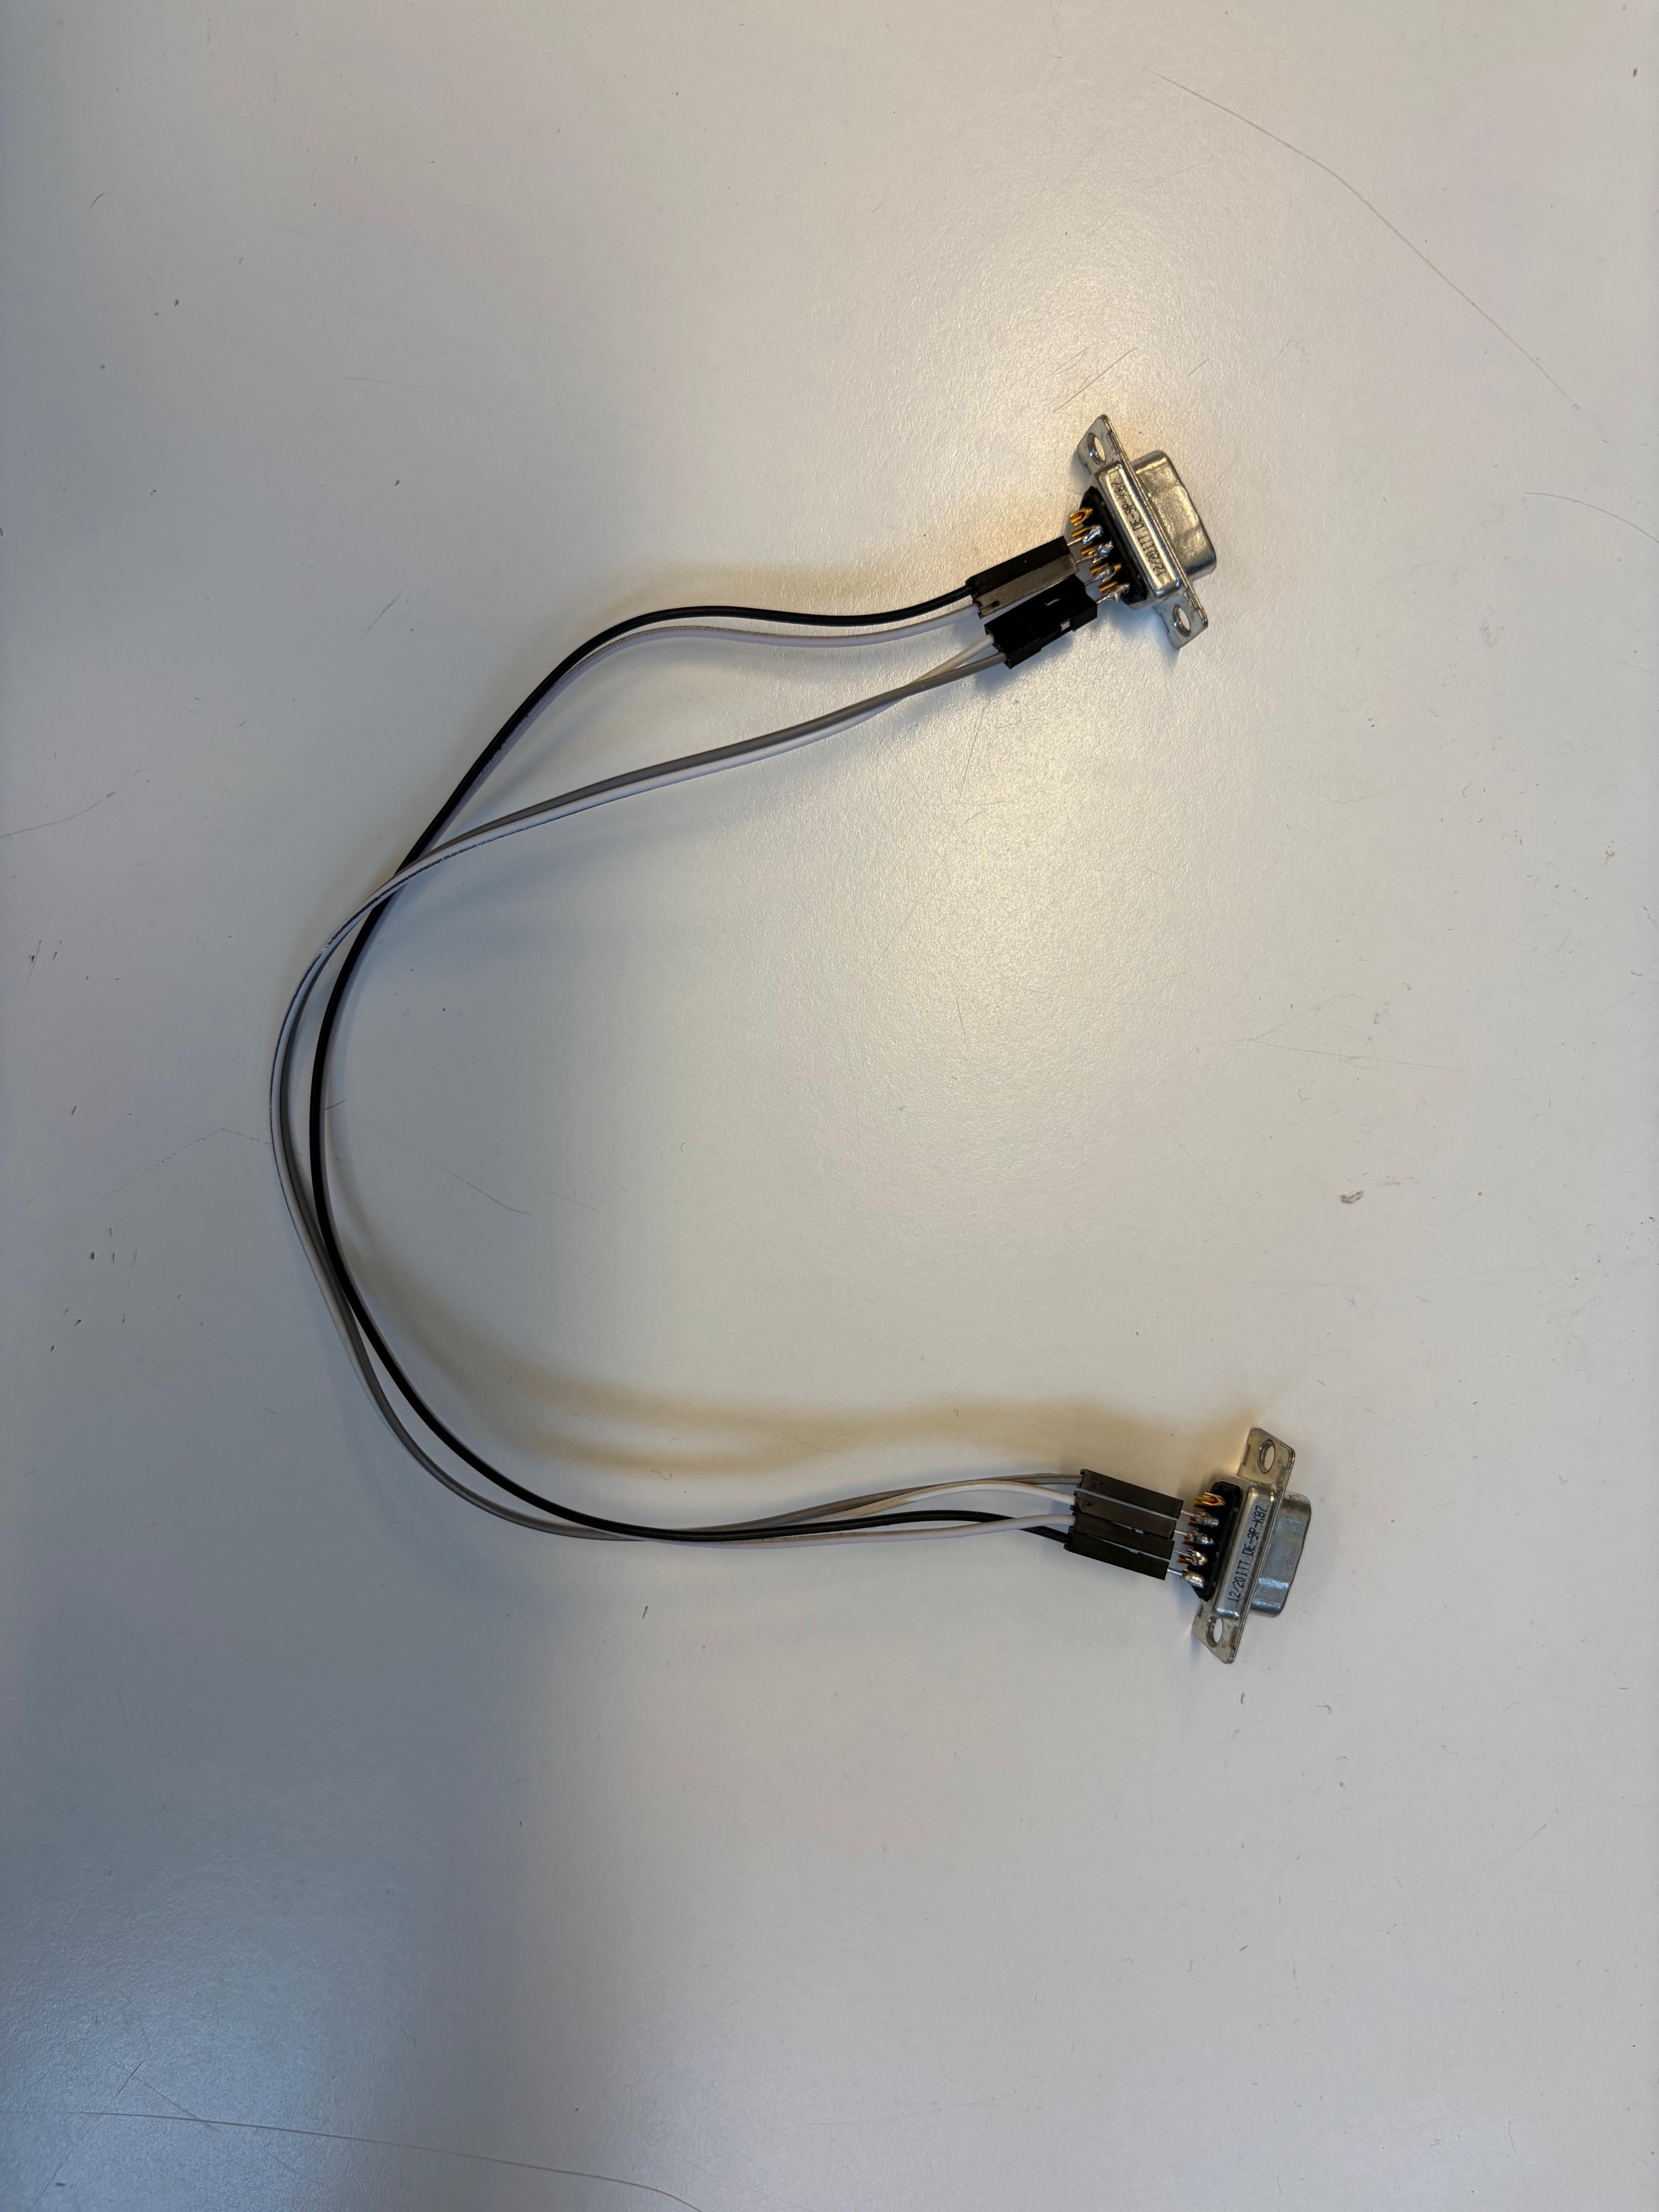
\includegraphics[width=\textwidth]{IMG/arnes_rs422.jpg}
        \caption{RS422, 4 hilos.}
        \label{fig:arnes_rs422}
    \end{subfigure}
    \hfill
    \begin{subfigure}[b]{0.32\textwidth}
        \centering
        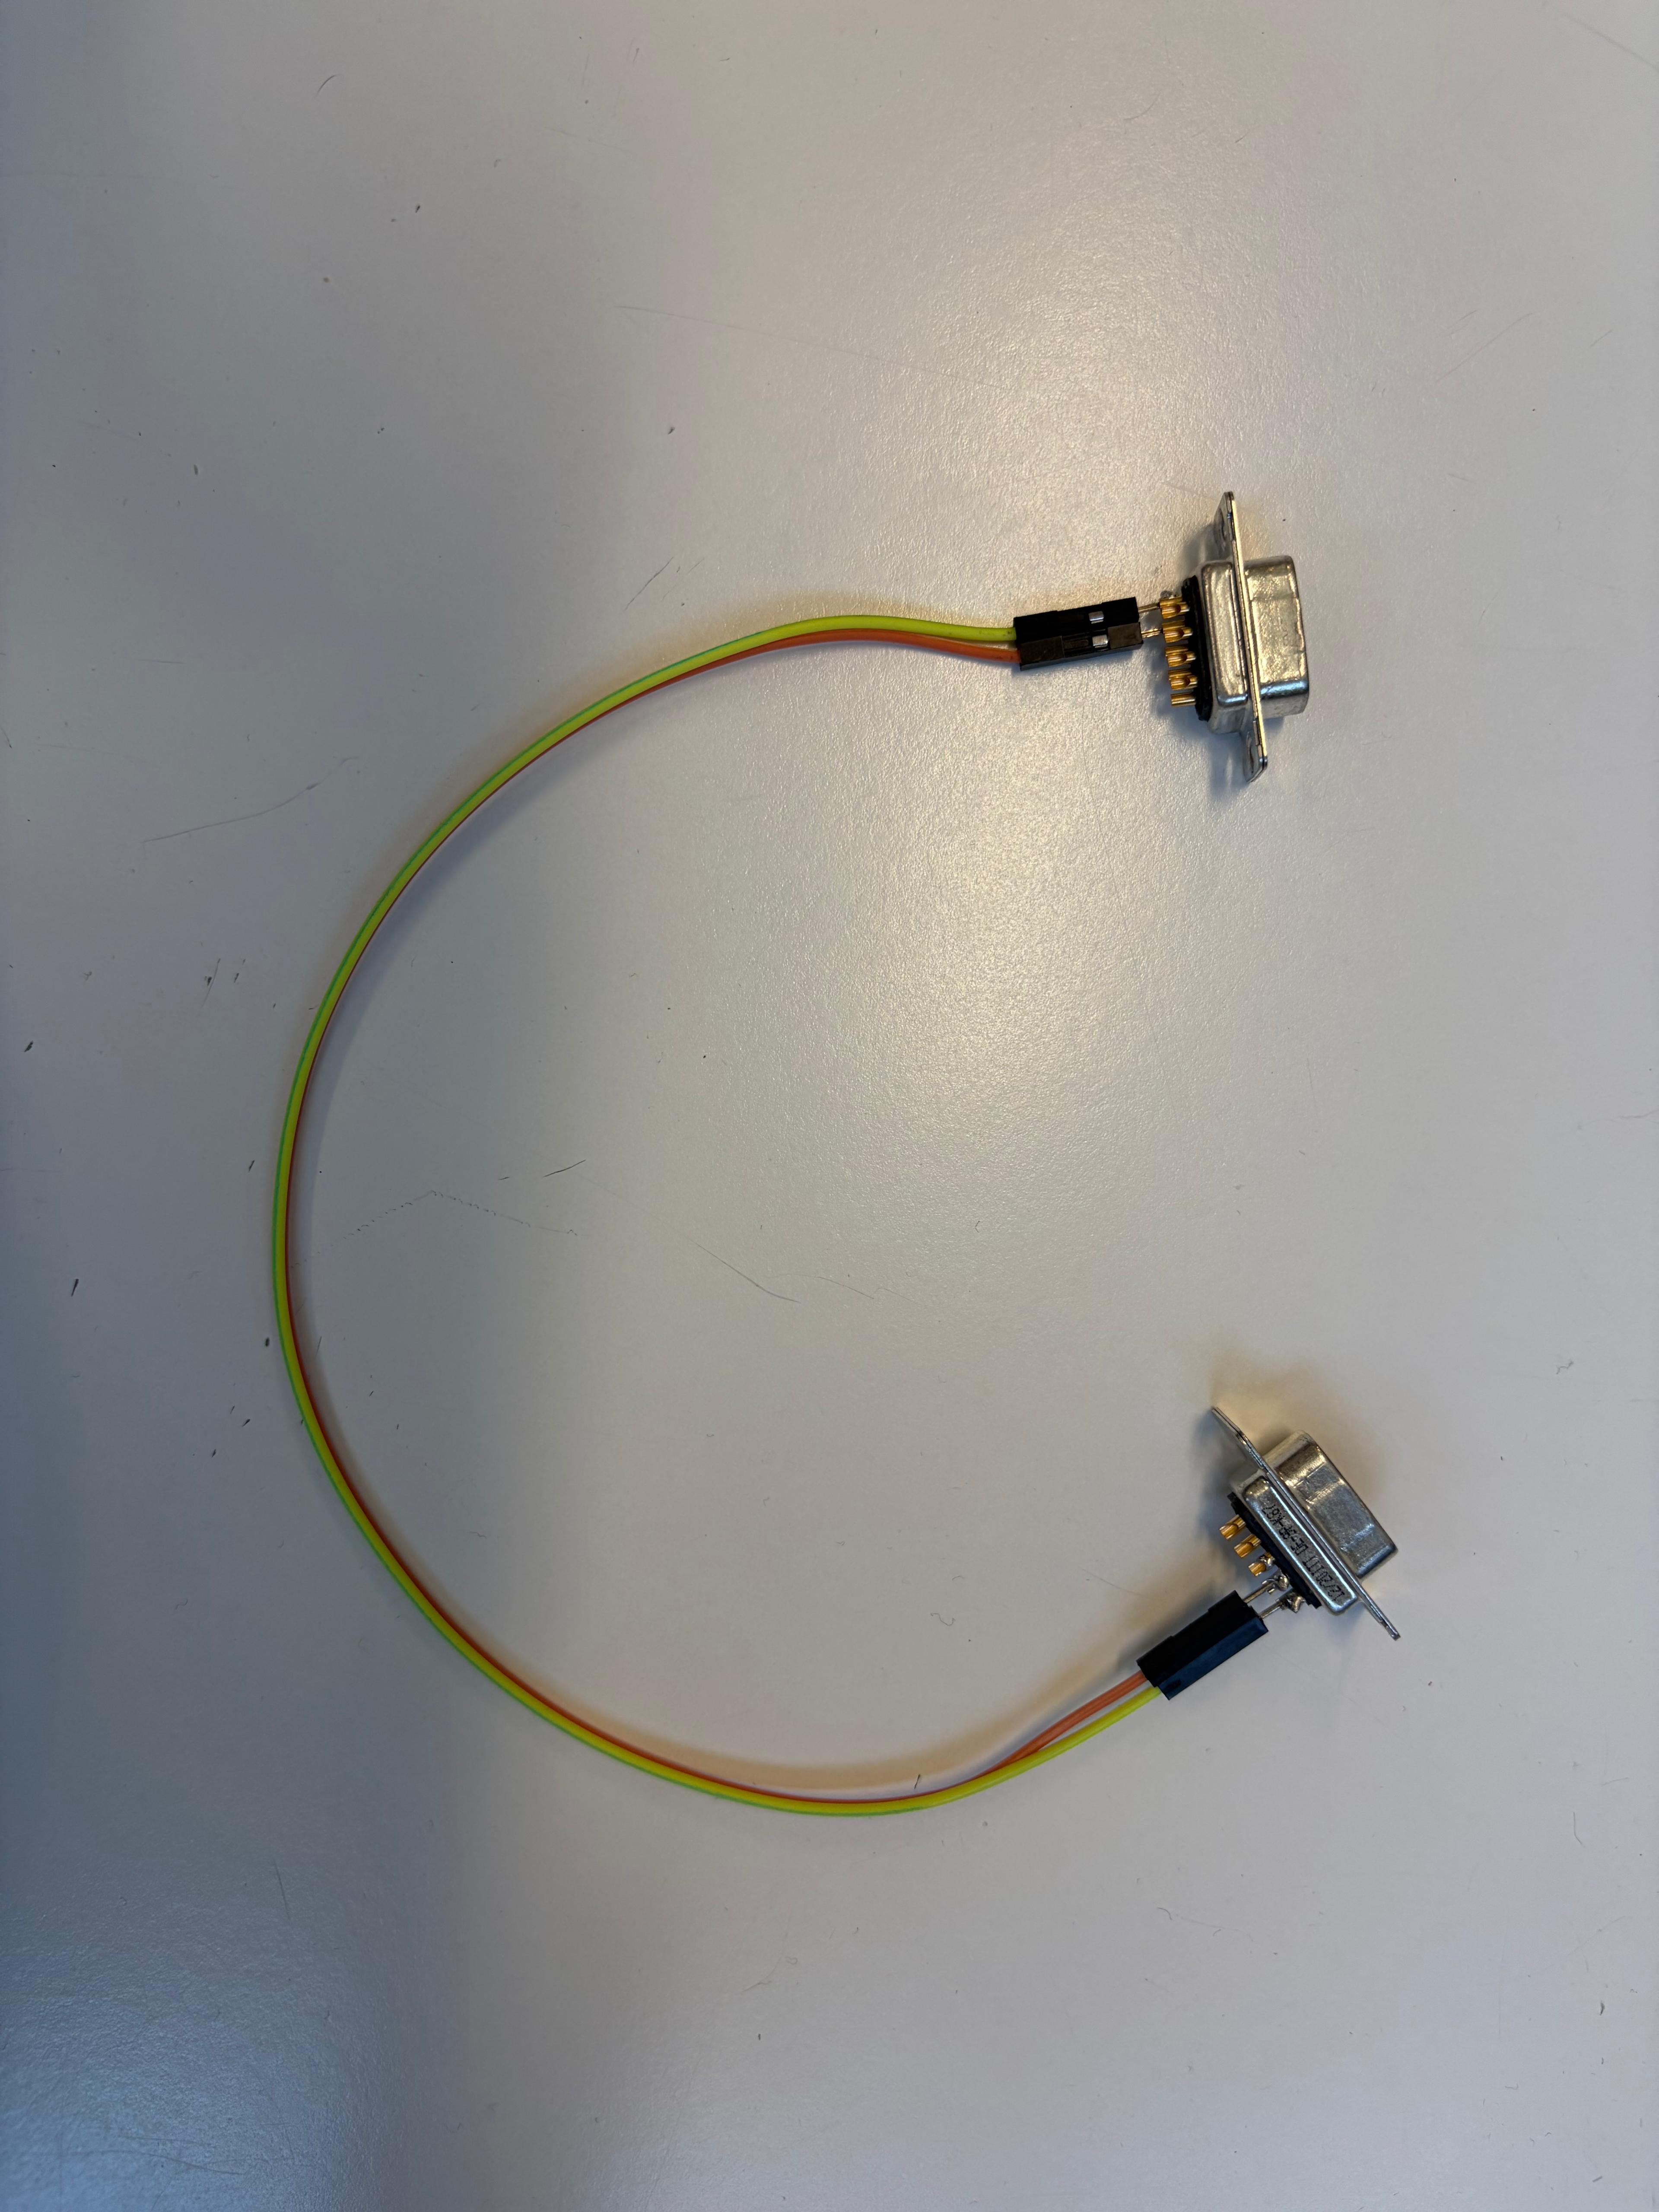
\includegraphics[width=\textwidth]{IMG/arnes_rs485.jpg}
        \caption{RS485, 2 hilos.}
        \label{fig:arnes_rs485}
    \end{subfigure}
    \hfill
    \begin{subfigure}[b]{0.32\textwidth}
        \centering
        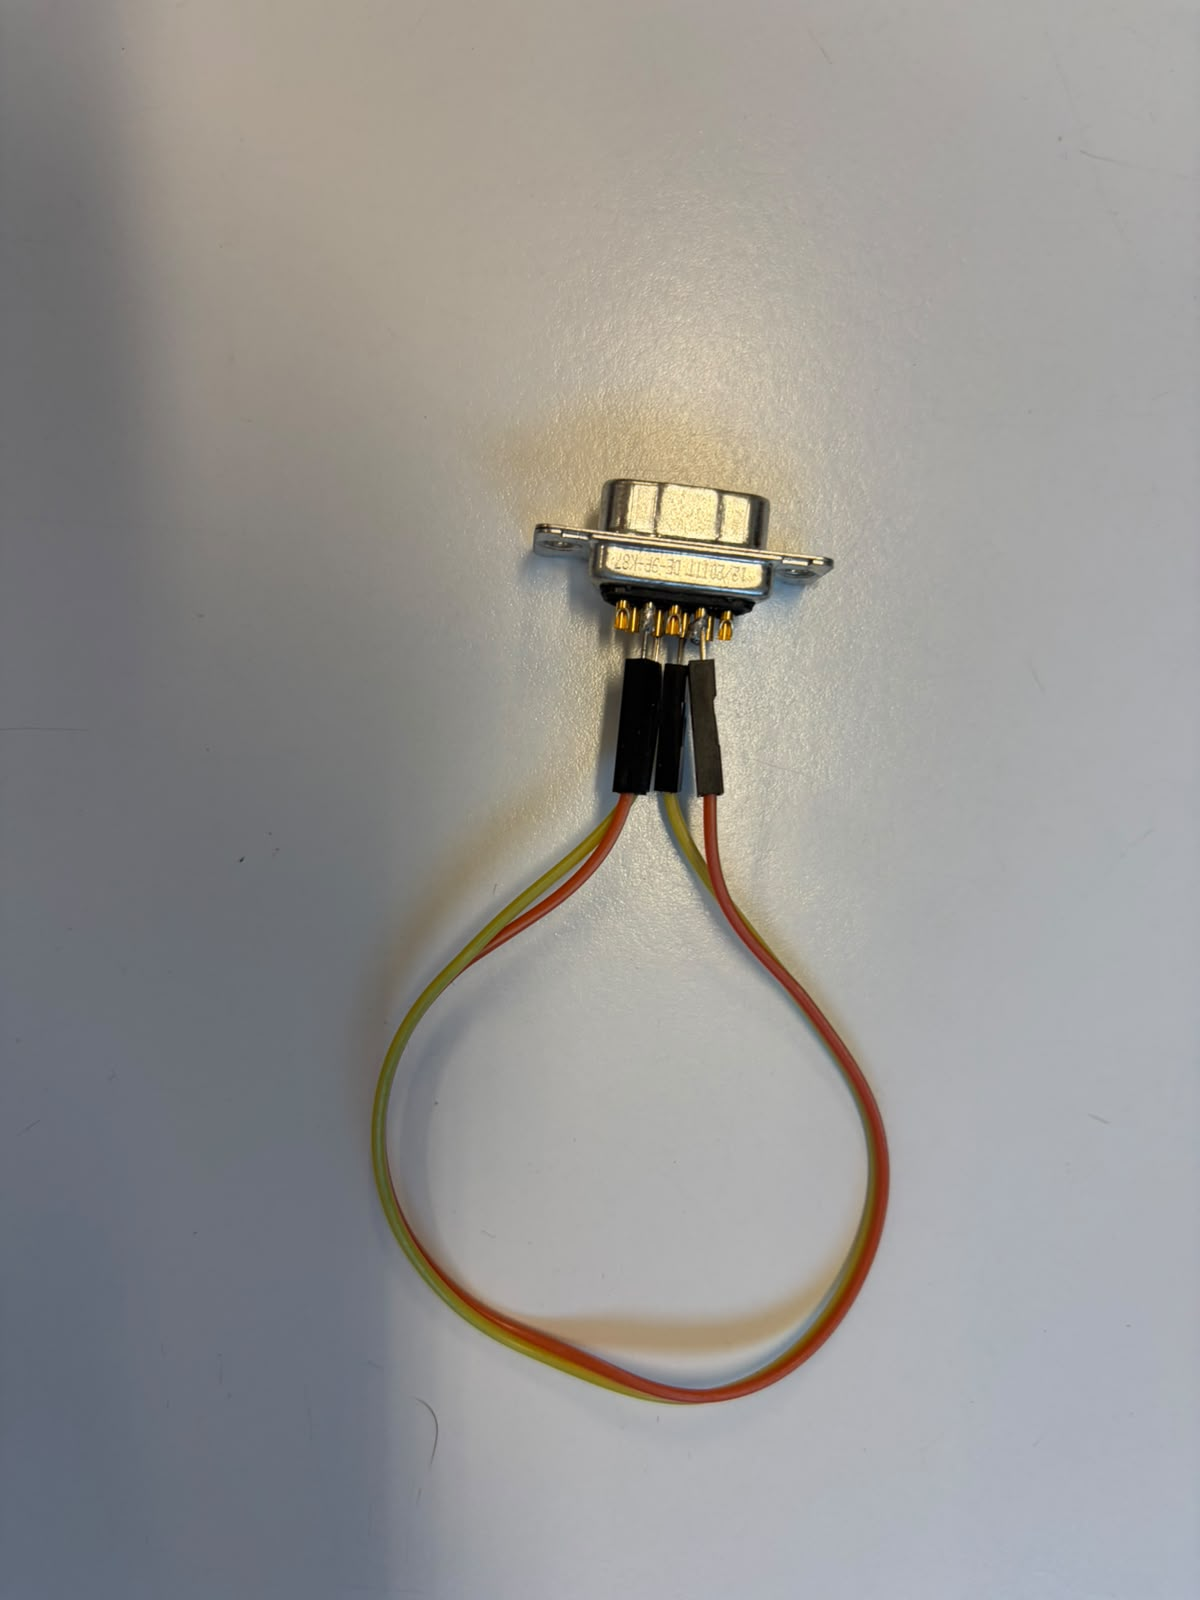
\includegraphics[width=\textwidth]{IMG/arnes_can.png}
        \caption{CAN nominal--redundante.}
        \label{fig:arnes_can}
    \end{subfigure}
    \caption{Arneses de \textit{loopback} sobre conector D-Sub-9.}
    \label{fig:arneses}
\end{figure}

\subsubsection{Equipo de laboratorio utilizado}

Se utilizó un osciloscopio y una fuente de alimentación de hasta 32~V.
